% Figure environments, with captions, for the three figures of one-loop diagrams that enter r0.
% Written for the one-column Supplement; the widths give the three figures the same scale.
% Suggested place: Sec. "One-loop correction to the DPS kernel", after the list of collinear diagrams.

\begin{figure}[t]
\centering
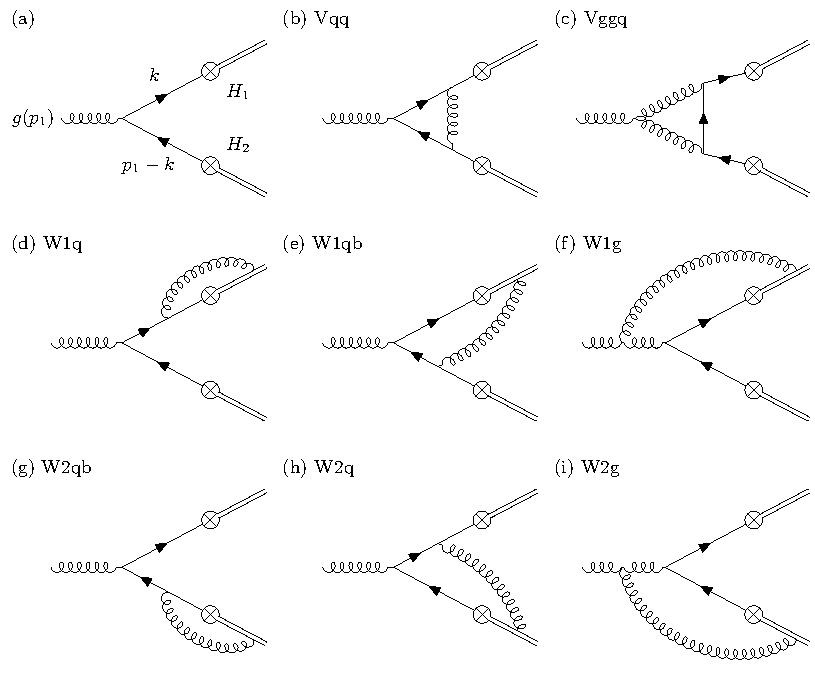
\includegraphics[width=0.72\textwidth]{figures/collinear_diagrams_qq.pdf}
\caption{One-loop diagrams of the collinear function $J_1$ for $g\to q\bar q$.
(a) Tree splitting. Crossed circles are the hard vertices $H_1$ and $H_2$ entered by
the quark, with momentum $k$, and the antiquark, with momentum $p_1-k$; double lines
are the Wilson lines of the two collinear fields.
(b) Abelian and (c) non-Abelian vertex corrections.
(d)--(f) Couplings of the Wilson line at $H_1$ to the quark, the antiquark and the
parent gluon. (g)--(i) Their mirror images for the Wilson line at $H_2$: couplings to
the antiquark, the quark and the parent gluon. Only (e) and (h) have a rapidity
divergence. Parton self-energy corrections are not shown. The labels are the names of the
diagrams in the accompanying repository.}
\label{fig:J1qq}
\end{figure}

\begin{figure}[t]
\centering
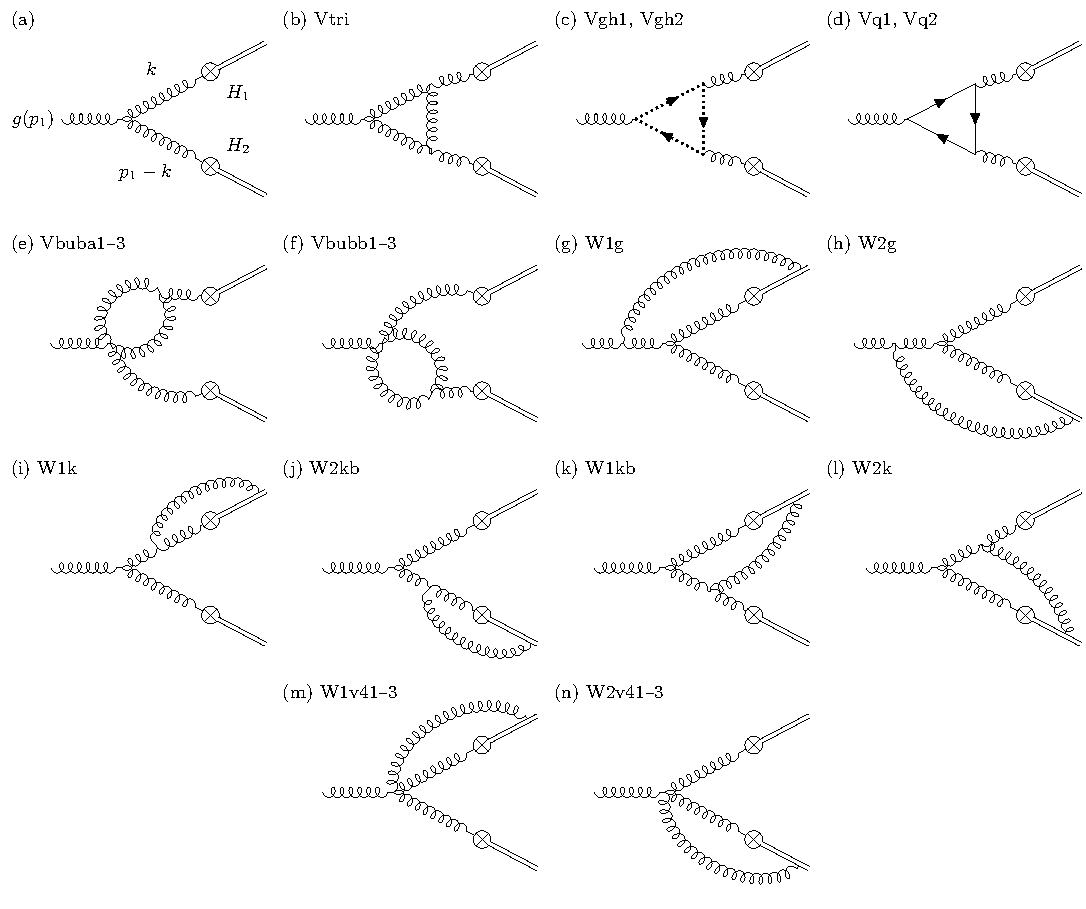
\includegraphics[width=0.96\textwidth]{figures/collinear_diagrams_gg.pdf}
\caption{One-loop diagrams of the collinear function $J_1$ for $g\to gg$, in the
notation of Fig.~\ref{fig:J1qq}. (a) Tree splitting. (b) Gluon, (c) ghost and
(d) quark triangles; both orientations of the ghost and quark loops are included.
(e), (f) Four-gluon vertex bubbles on either daughter.
(g), (h) Wilson line couplings to the parent gluon.
(i), (j) Wilson line couplings to the daughter entering the same hard vertex and
(k), (l) to the other daughter; only (k) and (l) have a rapidity divergence.
(m), (n) Diagrams in which the gluon from a Wilson line enters the four-gluon vertex.
These vanish in Feynman gauge. Parton self-energy corrections are not shown.}
\label{fig:J1gg}
\end{figure}

\begin{figure}[t]
\centering
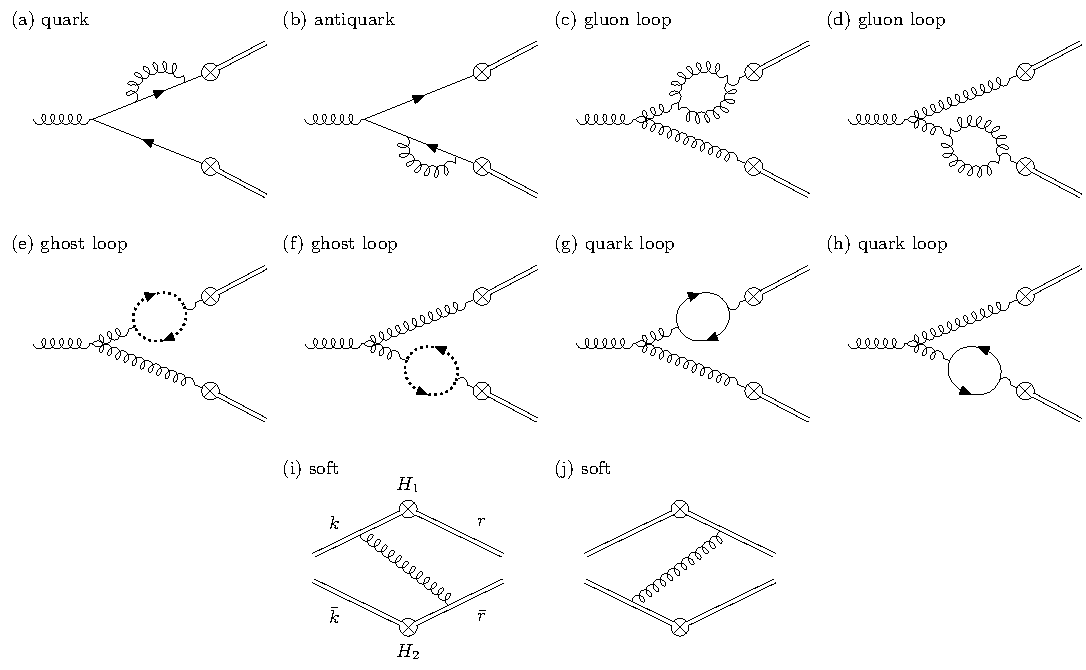
\includegraphics[width=0.96\textwidth]{figures/selfenergy_soft_diagrams.pdf}
\caption{Remaining one-loop contributions to $r_0$, in the notation of
Fig.~\ref{fig:J1qq}. (a), (b) Self-energy of the quark and of the antiquark for
$g\to q\bar q$. (c)--(h) Self-energy of a daughter gluon for $g\to gg$: gluon, ghost
and quark loops on either daughter. (i), (j) Soft exchanges between Wilson lines
entering different hard vertices, the two cross pairs $k,\bar r$ and $\bar k,r$.
Here $\bar k=p_1-k$, and $r$ and $\bar r$ are the daughters of the second incoming
gluon. An exchange within one hard vertex is scaleless, as is the self-energy of
an incoming gluon.}
\label{fig:r0rest}
\end{figure}
